% --------------------------------
% -------  chapter 10  ------------
% --------------------------------

\maketitle
\newpage
\section{Draw pictures}
  \textbf{
    The pgf/tikz package allows you to draw pictures from within your LaTeX document to keep the style consistent throughout your document.
  }
  \begin{enumerate} % list_type 有 enumerate、 itemize 和 description
    \item Basic example
    \item Syntax of tikz
  \end{enumerate} 
  The package pgf/tikz can be used to create beautiful graphics, especially diagrams in LaTeX. It enables you to create vector graphics from within your document, without the need of external tools such as Inkscape or Adobe Illustrator and thus is much more flexible. But unlike the graphical editors, we don't actually draw, but program the vector graphics using predefined macros. I will first show a little example using basic geometric elements and then explain the syntax of tikz.
  
  \subsection{A basic example}

  \begin{lstlisting}[language={[LaTeX]TeX},breaklines=true,frame=single]
    \documentclass{article}

    \usepackage{tikz}
    
    \begin{document}
    \begin{figure}[h!]
      \begin{center}
        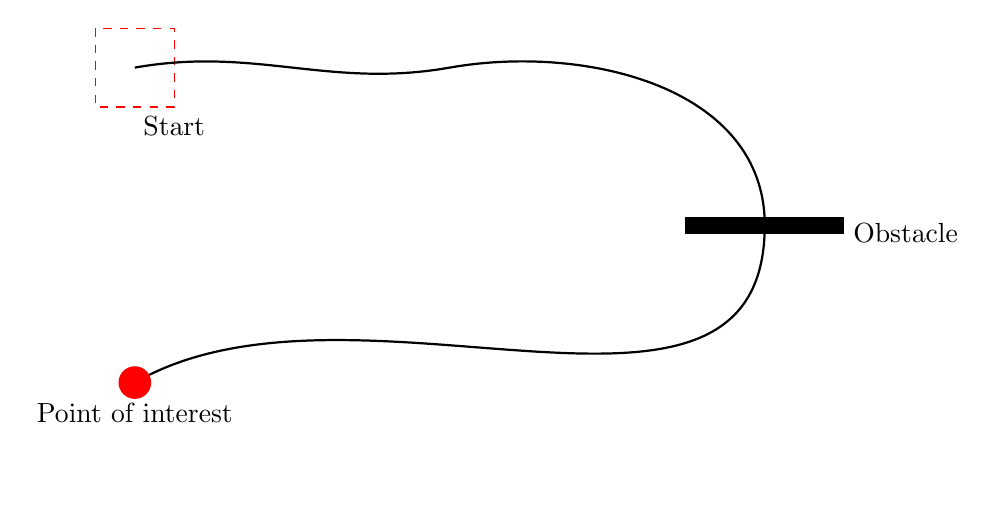
\begin{tikzpicture}
          \draw [red,dashed] (-2.5,2.5) rectangle (-1.5,1.5) node [black,below] {Start}; % Draws a rectangle
          \draw [thick] (-2,2) % Draws a line
          to [out=10,in=190] (2,2)
          to [out=10,in=90] (6,0) 
          to [out=-90,in=30] (-2,-2);    
          \draw [fill] (5,0.1) rectangle (7,-0.1) node [black,right] {Obstacle}; % Draws another rectangle
          \draw [red,fill] (-2,-2) circle [radius=0.2] node [black,below=4] {Point of interest}; % Draws a circle
        \end{tikzpicture}
        \caption{Example graphic made with tikz.}
      \end{center}
    \end{figure}
    \end{document}
  \end{lstlisting}
  \paragraph{}
  The result looks like this:
  \begin{figure}[h!]
    \begin{center}
      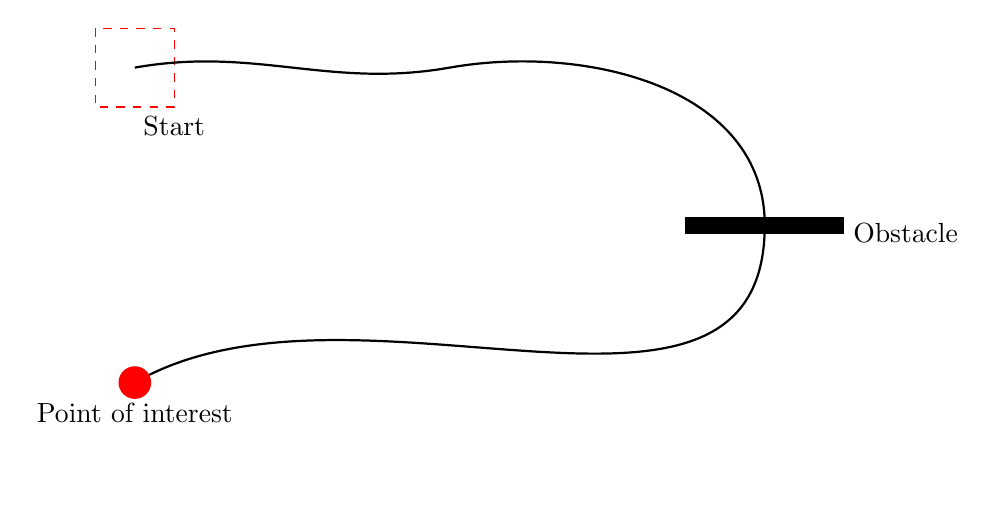
\begin{tikzpicture}
        \draw [red,dashed] (-2.5,2.5) rectangle (-1.5,1.5) node [black,below] {Start}; % Draws a rectangle
        \draw [thick] (-2,2) % Draws a line
        to [out=10,in=190] (2,2)
        to [out=10,in=90] (6,0) 
        to [out=-90,in=30] (-2,-2);    
        \draw [fill] (5,0.1) rectangle (7,-0.1) node [black,right] {Obstacle}; % Draws another rectangle
        \draw [red,fill] (-2,-2) circle [radius=0.2] node [black,below=4] {Point of interest}; % Draws a circle
      \end{tikzpicture}
      \caption{Example graphic made with tikz.}
    \end{center}
  \end{figure}

  \paragraph{}
  We usually want to embed our tikzpicture in a figure 
  environment. By using the \textbackslash draw command,
   we can add elements. It's necessary to specifiy 
   options in brackets and the coordinates of the element.


  \subsection{The syntax of Tikz}
  \paragraph{}
  To demonstrate the basic syntax, we will have a closer look at the line that draws the red rectangle in our picture:
  \begin{lstlisting}[language={[LaTeX]TeX},breaklines=true,frame=single]
    \draw [red,dashed] (-2.5,2.5) rectangle (-1.5,1.5) node [black,below] {Start};
  \end{lstlisting}
  \paragraph{}
  The options here indicate that the rectangle should be red and dashed, no magic here. Then we define the location of our rectangle (-2.5,2.5) in cartesian coordinates. To set the size of the rectangle, we simply add a second pair of coordinates behind our rectangle statement. (-1.5,1.5). As you can see, there is also a text below our rectangle. Text is usually placed as a so-called node (text-node) in our picture. We define the text to have black color and set the position to below our rectangle. Tikz can usually figure out the size of the rectangle automatically. Other than in plain LaTeX we have to terminate each command with a semicolon inside of the tikzpicture environment.
  \paragraph{}
  The next snippet shows how to draw a line by specifying a path in Tikz:
  \begin{lstlisting}[language={[LaTeX]TeX},breaklines=true,frame=single]
    \draw [thick] (-2,2) % Draws a line
    to [out=10,in=190] (2,2)
    to [out=10,in=90] (6,0) 
    to [out=-90,in=30] (-2,-2);   
  \end{lstlisting}
  \paragraph{}
  The syntax is the same as for the rectangle, we only use a different command in between the coordinates. The to command is used to specify a point of the path. Tikz usually draws straight lines between the points, in the picture below we can clearly see the lines are bent. This can be accomplished by setting the in and out angle in brackets. There are many more options available and mastering tikz can take a vast amount of time. Yet it is very easy to accomplish basic drawings very fast and they integrate very smoothly with the rest of your document. There are also many extensions for tikz, which provide easy ways to create diagrams, flowcharts, mindmaps and many more.

  \paragraph{Summary}
    % list
    \begin{itemize} % list_type 有 enumerate、 itemize 和 description
      \item Tikz can be used to draw graphics from within the LaTeX document
      \item No graphical user interface, instead pictures are programmed
      \item Extensive documentation available in the Tikz manual
      \item Many examples can be found on the internet
      \item Extensions available to easy creation of diagrams, flowcharts and so forth
    \end{itemize} 
